\chapter{Movement patterns}\label{movementpatterns}
%% Add figures!!

\section{Introduction}
The objective of this project is to identify movement patterns. To have a better understanding of this concept, it is important to describe relevant types of movement patterns in a systematic and comprehensive way. A classification of different patterns will provide guidelines for development of different mining algorithms and identify patterns. This chapter will first approach the definition of movement patterns. Subsequently, the theory is demonstrated with the research case of TU Delft in \autoref{movements}, \autoref{trajectories} and \autoref{indoormovement}. This illustrates what type of pattern mining methods can be used on a movement dataset. 

\section{Movement identification}
By definition, moving objects are entities whose positions of geometric attributes change over time (\citep{dodge2008towards}). People always move in geographic space, this means that human movement is geo-referenced. When the start and end time of one movement is specified, its trajectory can be constructed by ordering several movements of one individual. These trajectories can be visualized and analysed.

In order to identify movement patterns, it is important to understand what types of patterns may exist in the data. Besides, there are many types of patterns and not everything is relevant for this project. Therefore, this section will organize various categories. This project aims to identify three different movement patterns: \begin {enumerate*} [label=\itshape\arabic*\upshape),font={\color{red!0!black}\bfseries}] \item Spatio-temporal movement patterns; \item ordered co-location in space; \item unordered co-location in space. \end {enumerate*}\\\\
\textbf{Individual and group movement}\\
Patterns can occur in individual movements or in movements of a larger group. Typical movements of individuals will be different from typical movements of a larger group. For analyzing movement in a larger area with more than 25.000 users, we are interested in typical movement at the larger aggregate level of crowds. 

\subsection{Spatio-temporal movement patterns}
As described previous in this section, movement is from one location, or state, to another state, i.e. A to B. These movements can be analysed from movement data to detect the direct connectedness and flow between two locations in a time interval. Questions such as “where do people come from” and “how many people move between two locations” can be answered. Several patterns can be identified from this analysis. Firstly, the number of movements over time can be detected. This will provide insight in the behaviour of humans, e.g. when people go home or at what time people have lunch. Secondly, the flow and direction between two states, i.e. the analysis of the direction of the flows provides information on the symmetry of movement between two locations. For example, if 100 people move from A to B within a time interval and 100 people move from B to A in the same time interval, the movement pattern is perfectly symmetrical.
Besides analysing movements between two states, consecutive movements of one individual can be used to identify movement patterns. These trajectories will be the basis for the next section to identify co-locations of several trajectories. 	

\subsection{Co-location in space}
When moving individuals share some locations in their trajectory, you can speak of co-location in space. According to \citep{dodge2008towards} there are three types of co-location in space: \begin {enumerate*} [label=\itshape\arabic*\upshape),font={\color{red!0!black}\bfseries}] \item ordered co-location occurs when some locations are shared by multiple trajectories in the same order; \item unordered co-location when shared locations are attained in different orders; \item symmetrical co-location when the shared locations are in opposite order. This means that co-location in space, helps to identify movement patterns in the sense of frequently visited  locations in one trajectory. For example buildings A, B, C can be visited in the same order by multiple trajectories, and the same buildings can be visited by multiple trajectories, but in different orders. \autoref{figure:colocation} illustrates the concept of ordered co-location in space.
\end{enumerate*}

\begin{figure}[H]
\centering
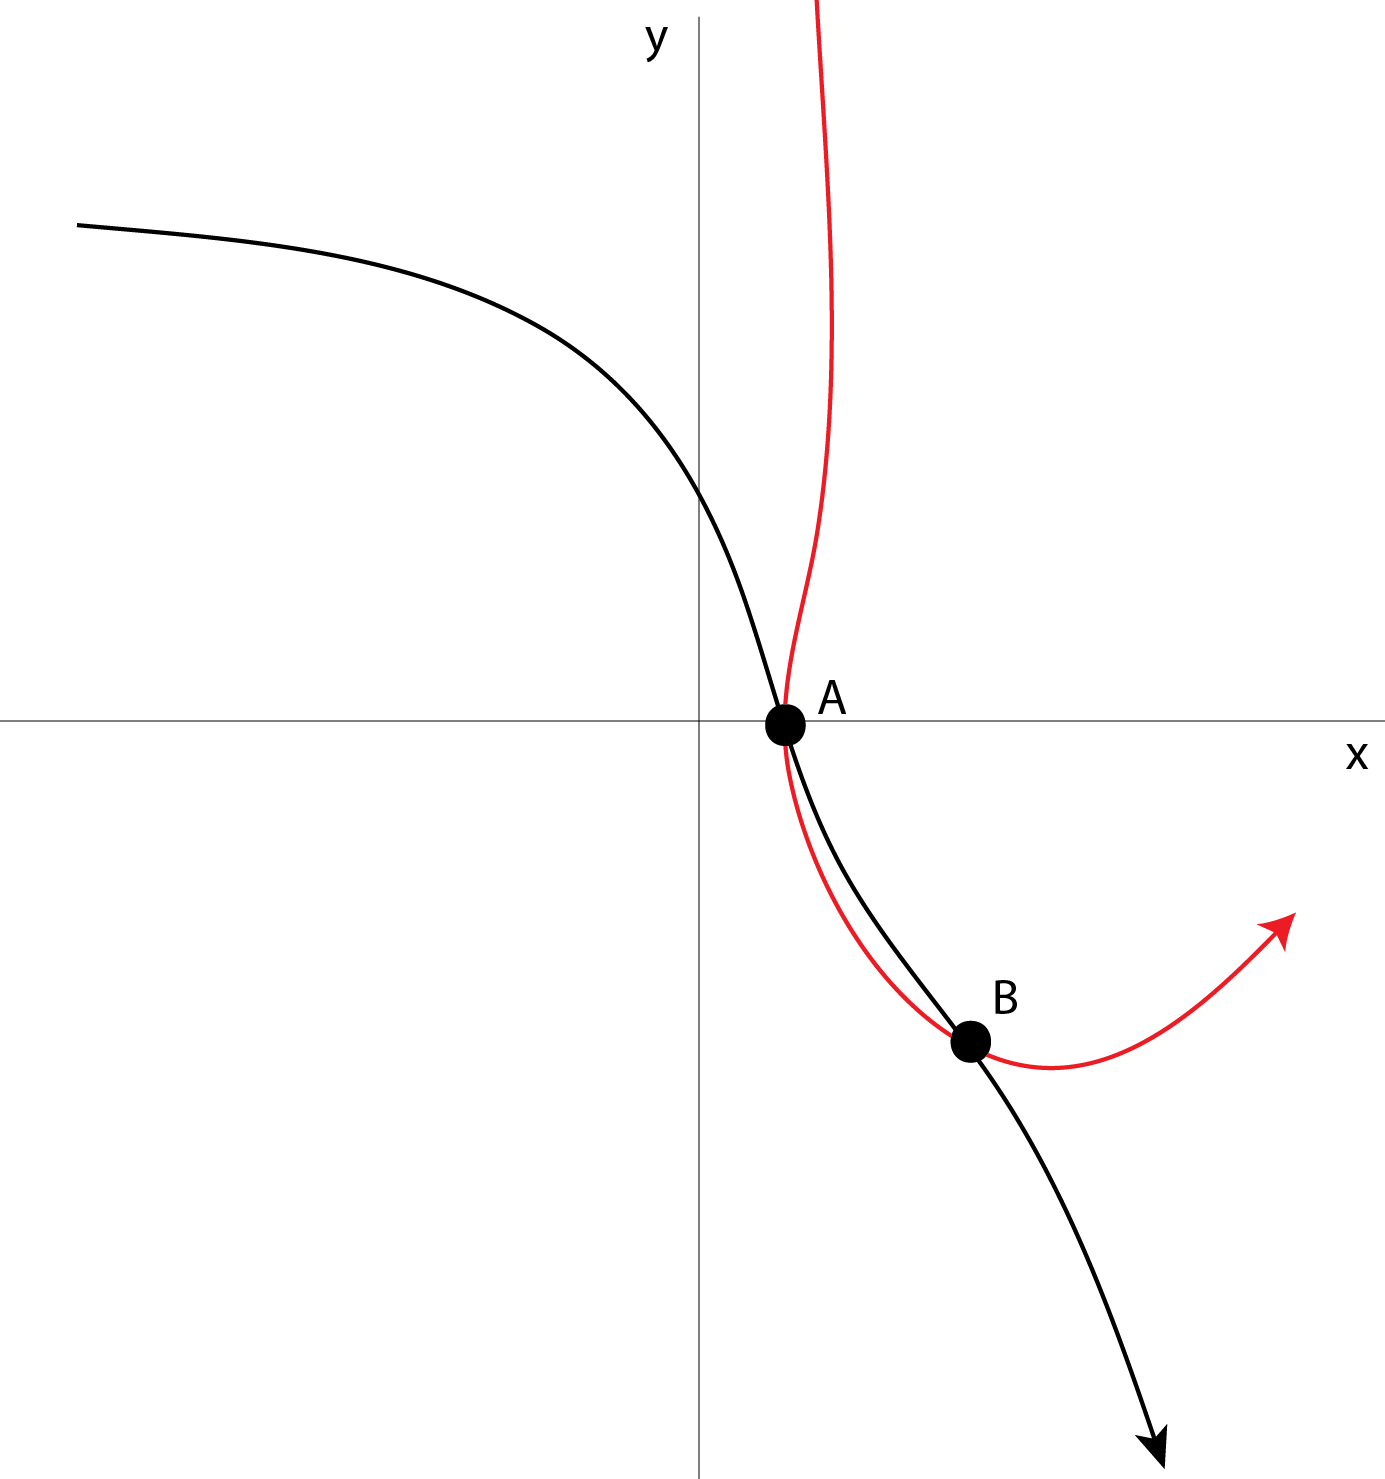
\includegraphics[scale=0.5]{ordered-co-location.png}
\captionsetup{justification=centering}
\caption{Ordered co-location in space}
\label{figure:colocation}
\end{figure}

Ordered co-location is space can be analysed with the concept of sequences. A sequence is an ordered list of visited locations. Sequential pattern mining algorithm help to understand a what order common locations are visited. In this report, trajectories of a sequence of locations are analysed to identify ordered co-location in space movement patterns.
Unordered co-location in space analyses the same trajectories, but does not consider direction or order of the movement. This means that common locations visited together in one trajectory can be identified. In other words, the association between buildings is detected. A commonly used method to detect groups of objects in a list (i.e. a trajectory), an association rule mining algorithm can used. Our research did not include this in the final results, but this report will elaborate on the concept of this algorithm in \autoref{dist_usergroups}.